\section{Introduction}

When working with polygonal and polyhedral sets, the mathematical
model determines the kind of point set that can be represented. Nef
polyhedra are the most general rectilinear polyhedral model.

Topological simpler models that are contained in the domain of
Nef polyhedra are:
\begin{itemize}
\item \emph{convex polytopes} normally defined as the convex hull
  of a nonempty finite set of points. Convex polytopes are 
  compact closed and manifold sets. 
\item \emph{elementary polyhedra} normally defined as the union
  of a finite number of convex polytopes. 
\item \emph{polyhedral sets} nomally defined as the intersection
  of a finite number of closed halfspaces. Such sets are closed and
  convex but need not to be compact. 
\item \emph{linear polyhedra} normally defined as the set of all
points belonging to the simplices of a \emph{simplicial complex}. 
\end{itemize}

A planar \emph{Nef polyhedron} is any set that can be obtained from a
finite set of open halfspaces by set complement and set intersection
operations. Due to the fact that all other binary set operations like
union, difference and symmetric difference can be reduced to
intersection and complement calculations, Nef polyhedra are also closed
under those operations. Apart from the set complement operation there
are more topological unary set operations that are closed in the
domain of Nef polyhedra. Given a Nef polyhedron one can determine its
interior, its boundary, and its closure, and also composed operations
like regularization (defined to be the closure of the interior or a
point set).

\begin{figure}[htbp]
\begin{ccTexOnly}
\begin{center}
\scalebox{0.5}{\includegraphics{halfplane.ps}}
\hspace{1cm}
\scalebox{0.5}{\includegraphics{complex.ps}}
\end{center}
\end{ccTexOnly}
\caption{Two Nef polyhedra in the plane. A closed halfspace on the 
left and a complex polyhedron on the right. Note that the points 
on the squared boundary are at infinity.}\label{nefexamples}
\begin{ccHtmlOnly}
<CENTER>
<IMG BORDER=0 SRC="./halfplane.gif" ALIGN=center
ALT="a halfplane">
<IMG BORDER=0 SRC="./complex.gif" ALIGN=center
ALT="a complex polyhedron">
</CENTER>
\end{ccHtmlOnly}
\end{figure}      

\section{Construction and Composition}

Following the above definition, the data type
\ccc{Nef_polyhedron_2<T>} allows construction of elementary Nef
polyhedra and the binary and unary composition by the mentioned set
operations.

In the following examples skip the typedefs at the beginning at first
and take the types \ccc{Point} and \ccc{Line} to be models of the
standard two-dimensional CGAL kernel (\ccc{CGAL::Point_2<K>}
and \ccc{CGAL::Line_2<K>}). Their user interface is thus defined in
the corresponding reference pages.

\ccIncludeExampleCode{Nef_2/construction.C}

Planar halfspaces (as used in the definition) are modelled by oriented
lines. In the previous example \ccc{N1} is the Nef polyhedron
representing the full plane, \ccc{N2} is the closed halfspace left of
the oriented line with equation $2x + 4y + 2 = 0$ including the line,
\ccc{N3} is the complement of \ccc{N2} and therefore it must hold that
$N2 \cup N3 = N1$.

Additionally one can construct Nef polyhedra from iterator ranges that
hold simple polygonal chains. In the example \ccc{N4} is the triangle
spanned by the vertices $(0,0)$, $(10,10)$, $(-20,15)$.  Note that the
construction from a simple polygonal chain has several cases and
preconditions that are described in the reference manual page of
\ccc{Nef_polyhedron_2<T>}. The \ccc{operator<=} in the last assertion
is a subset-or-equal comparison of two polyhedra.

Nef polyhedra have input and output operators that allows one to
output them via streams and read them from streams. Graphical output
is currently possible to a \ccc{CGAL::Window_stream}. The output
operation is defined in
\ccc{CGAL/IO/Nef_polyhedron_2_Window_stream.h}. For an elaborate
example see the demo programs in the directory \ccc{demo/Nef_2}.

\section{Exploration}

By recursively composing binary and unary operations one can end with
a very complex rectilinear structure. To explore that structure there
is a data type \ccc{Nef_polyhedron_2<T>::Explorer} that allows
read-only exploration of the rectilinear structure. To understand its
usability we need more knowledge about the representation of Nef
polyhedra.

The rectilinear structure underlying a Nef polyhedron is stored in a
selective plane map. Plane map here means a straightline embedded
bidirected graph with face objects such that each point in the plane
can be uniquely assigned to an object (vertex, edge, face) of the
planar subdivision defined by the graph. Selective means that each
object (vertex, edge, face) has a Boolean value associated with it to
indicate set inclusion or exclusion.

The plane map is defined by the interface data type
\ccc{Nef_polyhedron_2<T>::Topological_explorer}. Embedding the vertices by
standard affine points does not suffice to model the unboundedness of
halfspaces and ray-like structures. Therefore the planar subdivision
is bounded symbolically by an axis-parallel square box of infimaximal
size centered at the origin of our coordinate system. All structures
extending to infinity are pruned by the box. Lines and rays have
symbolic endpoints on the box. Faces are circularly closed.
Infimaximal here means that its geometric extend is always large
enough (but finite for our intuition). Assume you approach the box
with an affine point, then this point is always inside the box. The
same holds for straight lines; they always intersect the box. There
are more accurate notions of ``large enough'', but the previous
propositions are enough at this point. Due to the fact that the
infimaximal box is included in the plane map, the vertices and edges
are partitioned with respect to this box.

Vertices inside the box are called standard vertices and they are
embedded by affine points of type \ccc{Explorer::Point}. Vertices on
the box are called non-standard vertices and they get their embedding
where a ray intersects the box (their embedding is defined by an
object of type \ccc{Explorer::Ray}). By their straightline embedding,
edges represent either segments, rays, lines, or box segments
depending on the character of their source and target vertices.

During exploration, box objects can be tracked down by the interface
of \ccc{Nef_polyhedron_2<T>::Explorer} that is derived from
\ccc{Nef_polyhedron_2<T>::Topological_explorer} and adds just the box
exploration functionality to the interface of the latter. In the
following code fragment we iterate over all vertices of a Nef
polhedron and check whether their embedding is an affine point or a
point on the infimaximal frame.
\begin{ccExampleCode}
typedef Nef_polyhedron::Explorer Explorer;
Explorer E = N4.explorer();
Explorer::Vertex_const_iterator v;
for (v = E.vertices_begin(); v != E.vertices_end(); ++v)
  if ( E.is_standard(v) ) 
    Explorer::Point p = E.point(v) // affine embedding of v
  else /* non-standard */ 
    Explorer::Ray r = E.ray(v) // extended embedding of v
\end{ccExampleCode}

Note that box edges only serve as boundary edges (combinatorically) to
close the faces that extend to infinity (geometrically). Their status
can be queried by the following operation:
\begin{ccExampleCode}
typedef Nef_polyhedron::Explorer Explorer;
Explorer E = N4.explorer();
Explorer::Halfedge_const_iterator e;
for (e = E.halfedges_begin(); e != E.halfedges_end(); ++e)
  if ( E.is_frame_edge(e) ) // e is part of square box.
\end{ccExampleCode}

\section{Traits Classes}

Now finally we clarify what the template parameter of class
\ccc{Nef_polyhedron_2<T>} actually models. \ccc{T} carries the
implementation of a so-called extended geometric kernel.

Currently there are three kernel models:
\ccc{CGAL::Extended_cartesian<FT>},
\ccc{CGAL::Extended_homogeneous<RT>}, and
\ccc{CGAL::Filtered_extended_homogeneous<RT>}. The latter is the most
optimized one. The former two are simpler versions corresponding to
the simple planar affine kernels.  Actually, it holds that (type
equality in pseudo-code notation):
\begin{ccExampleCode}
CGAL::Nef_polyhedron_2< CGAL::Extended_cartesian<FT> >::Point 
  == CGAL::Cartesian<FT>::Point_2

CGAL::Nef_polyhedron_2< CGAL::Extended_homogeneous<RT> >::Point
   == CGAL::Homogeneous<RT>::Point_2

CGAL::Nef_polyhedron_2< CGAL::Filtered_extended_homogeneous<RT> >::Point
   == CGAL::Homogeneous<RT>::Point_2
\end{ccExampleCode}
Similar equations hold for the types \ccc{Line} and \ccc{Direction} in
the local scope of \ccc{Nef_polyhedron_2<...>}.

\begin{ccAdvanced}
For its notions and requirements see the desciption of the concept
\ccc{ExtendedKernelTraits_2} in the reference manual.
\end{ccAdvanced}

\section{Implementation}

The underlying set operations are realized by an efficient and
complete algorithm for the overlay of two plane maps. The algorithm is
efficient in the sense that its running time is bounded by the size of
the inputs plus the size of the output times a logarithmic factor. The
algorithm is complete in the sense that it can handle all inputs and
requires no general position assumption.



